\documentclass[titlepage]{article}
\usepackage{amsmath}
\usepackage[capitalise, dutch]{cleveref}
\usepackage[labelfont=bf]{caption}
\usepackage{subcaption}
\usepackage{graphicx}
\usepackage[outdir=../plots/]{epstopdf}
\usepackage[section]{placeins}
\usepackage[backend=biber,citestyle=numeric,style=ieee]{biblatex}
\usepackage{siunitx}
\usepackage[main=dutch]{babel}
\usepackage{geometry}
\usepackage{float}
\usepackage{derivative}
\usepackage[T1]{fontenc}

\graphicspath{{../plots/}}
\addbibresource{bibliography.bib}
\sisetup{output-exponent-marker=\ensuremath{\mathrm{e}}}

\title{Theorie \& praktijk van eindige elementen methoden: programmeeropdracht}
\author{Othman El Hammouchi}

\begin{document}

\begin{titlepage}
  \maketitle
\end{titlepage}

De functie \texttt{fem\_solve} in het bestand \texttt{helpers.py} implementeert een eindige elementen-methode
voor het oplossen van de eendimensionale diffusievergelijking
\begin{equation} \label{eq:heat}
  -k \odv[order=2]{T}{x} = q \,,
\end{equation}
die de hitte beschrijft in een staaf van niet-homogeen materiaal. Het oplossingsdomein wordt verkregen op de wijze die in de opdracht geschetst werd, en de randvoorwaarden zijn $T(0) = 100$ en $\odv{T}{x}_{L} = 0$. De analytische oplossing wordt berekend in de functie \texttt{exact\_solve}, en het bestand \texttt{main.py} bevat code om de twee grafisch te vergelijken en een empirische foutanalyse uit te voeren. Teneinde grotere algemeenheid te verkrijgen worden de elementen en knopen zoals gevraagd gepermuteerd alvorens ze in de hoofdlus van de solver belanden; \cref{tab:elems,tab:nodes} tonen de eerste 10 elementen en knopen die op deze manier verkregen werden. \Cref{fig:sol-plot} vergelijkt de exact en eindige elementen-oplossingen, en hieruit blijkt duidelijk dat het verschil tussen beiden minimaal is, hetgeen de nauwkeurigheid van de numerieke oplossingsmethode illustreert. De benadering van de gradi\"ent, die in \cref{fig:grad-plot} weergegeven wordt, vertoont een verloop dat overeenkomt met onze verwachtingen: het is stuksgewijs constant in de gebieden zonder warmteproductie ten gevolge van de verschillende materiaalconstanten, en stijgt/daalt lineair op de intervallen waar warmte wordt toegevoegd. Tenslotte bevat \cref{fig:error-plot} een dubbellogaritmische weergave van de gemiddelde kwadratische fout, en dit verschaft een empirische bevestiging van de tweedeordenauwkeurigheid van deze methode: we zien dat de fout met tweede ordegroottes afneemt wanneer de elementbreedte met \'e\'en ordegrootte wordt gereduceerd.

\begin{figure}[!htb]
  \begin{displaymath}
    \begin{matrix}
  2197.00 &  3436.00 &  30.78 &  0.00\\
  10133.00 &  6864.00 &  30.78 &  0.00\\
  6700.00 &  9740.00 &  18.97 &  0.00\\
  7810.00 &  8184.00 &  15.33 &  10.00\\
  5237.00 &  498.00 &  11.90 &  0.00\\
  4603.00 &  3813.00 &  26.71 & -3.90\\
  5741.00 &  8737.00 &  30.78 &  0.00\\
  5185.00 &  216.00 &  17.13 &  0.00\\
  5548.00 &  1848.00 &  15.33 &  10.00\\
  10190.00 &  3914.00 &  11.90 &  0.00
\end{matrix}    
  \end{displaymath}
  \caption{Eerste 10 elementen}
  \label{tab:elems}
\end{figure}

\begin{figure}[!htb]
  \begin{displaymath}
    \begin{matrix}
  93.82 &  98.34 &  20.13 &  93.72 &  46.09 &  83.01 &  13.64 &  14.16 &  10.69 &  62.35
\end{matrix}
  \end{displaymath}
  \caption{Eerste 10 knopen}
  \label{tab:nodes}
\end{figure}

\begin{figure}[!p]
  \begin{subfigure}{\linewidth}
    \centering
    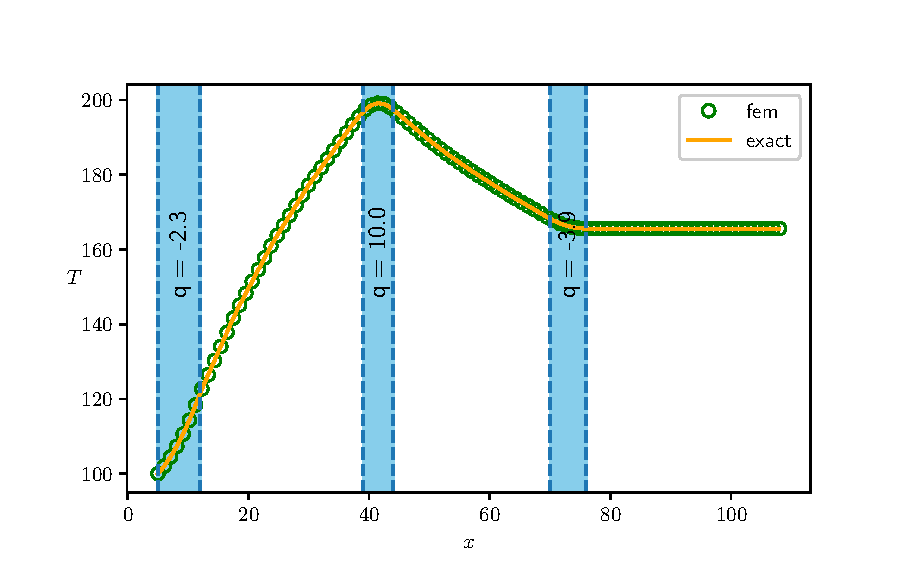
\includegraphics{sol}
    \subcaption{Exacte en eindige elementen-oplossing}
    \label{fig:sol-plot}
  \end{subfigure}
  \begin{subfigure}{\linewidth}
    \centering
    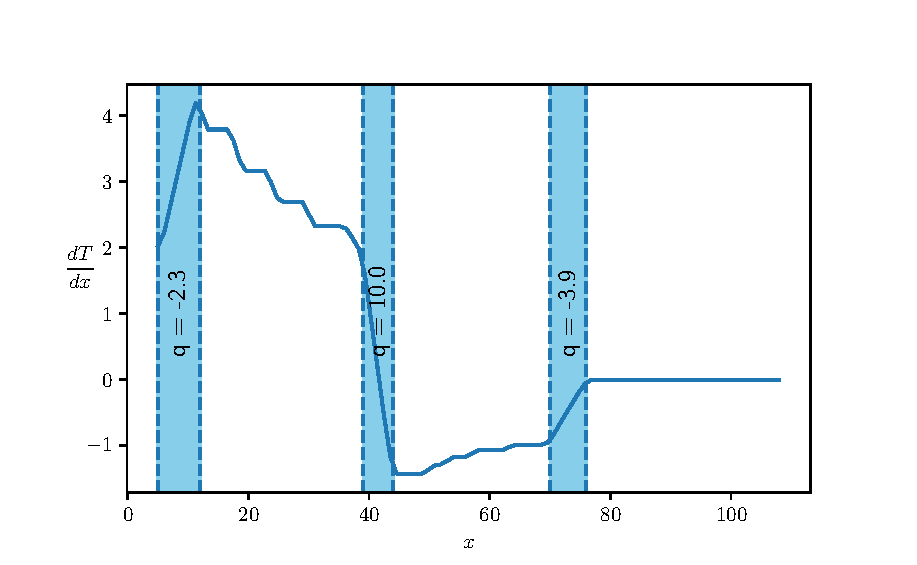
\includegraphics{grad}
    \subcaption{Benadering van de gradi\"ent}
    \label{fig:grad-plot}
  \end{subfigure}
  \caption{Grafieken verkregen bij de oplossing van \cref{eq:heat}. De lichtblauwe stroken duiden de gebieden aan waarin warmte wordt toegevoegd.}
\end{figure}

\begin{figure}[!htb]
  \centering
  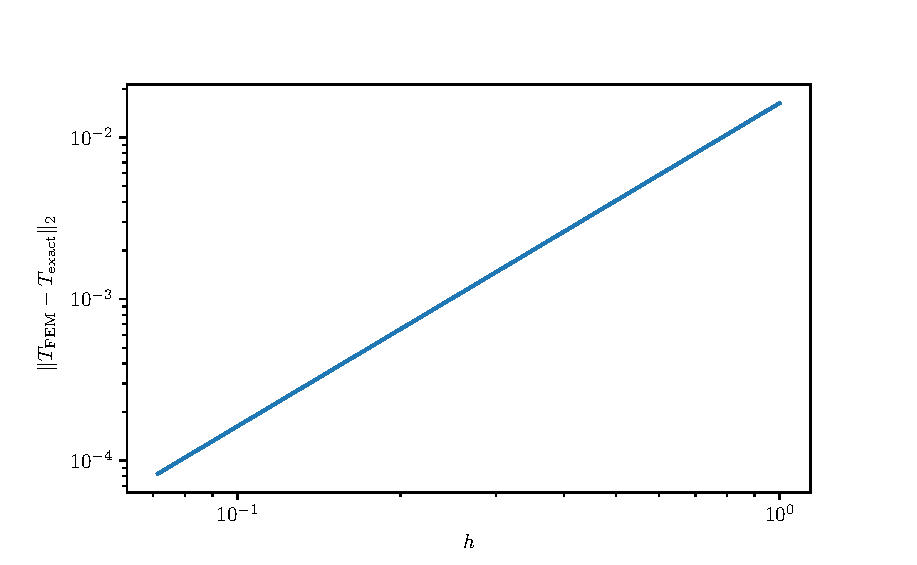
\includegraphics{error}
  \caption{Dubbellogaritmische weergave van de fout als functie van de elementgrootte}
  \label{fig:error-plot}
\end{figure}

\end{document}